
%%%%%%%%%%%%%%%%%%%%%%% file LatexExample.tex %%%%%%%%%%%%%%%%%%%%%
%
% This is the LaTeX source for the instructions to authors using
% the LaTeX document class 'llncs.cls'.
% http://www.springer.com/lncs       Springer Heidelberg 2006/05/04
%
% It may be used as a template for your own input - copy it
% to a new file with a new name and use it as the basis
% for your article.
%
% NB: The document class 'llncs' has its own and detailed documentation, see
% ftp://ftp.springer.de/data/pubftp/pub/tex/latex/llncs/latex2e/llncsdoc.pdf
%
%%%%%%%%%%%%%%%%%%%%%%%%%%%%%%%%%%%%%%%%%%%%%%%%%%%%%%%%%%%%%%%%%%%


\documentclass[runningheads,a4paper]{llncs}

\input{settings}

%------------------------- BEGIN DOCUMENT -------------------------%
\begin{document}

\mainmatter  % Start of an individual contribution

% TITLE
\title{Report on Fast Approximate Energy Minimization via Graph Cuts}


% A short form should be given in case it is too long for the running head
\titlerunning{Paper Report}


% AUTHORS
\author{%
Felix Wechsler\\Technische Universit{\"a}t M{\"u}nchen, Germany \\ \href{mailto:felix.wechsler@tum.de}{felix.wechsler@tum.de}%
} 

% Running header author
\authorrunning{Felix Wechsler}
% AFFILIATION
% \institute{%
% Departments of Informatics, Technische Universit{\"a}t M{\"u}nchen, Germany, \email{felix.wechsler@tum.de}%
% }
\institute{lol}
% \toctitle{Report about Fast Approximate Energy Minimization via Graph Cuts}
% \tocauthor{Felix Wechsler}
\maketitle

%------------------------- ABSTRACT -------------------------%
% \begin{abstract}
% In the following report we want to give an introduction about graph cuts which are used in computer vision.
% Our report is based on \cite{paper} which introduces a fast approximate way of minimizing the energy in a image.
% A simple proof-of-concept implementation - written in \texttt{Python} - is used to show the behaviour in image restoration using different energy functions.
% \keywords{Energy Minimizing Graph Cuts} % Optional
% \end{abstract}

%------------------------- SECTIONS -------------------------%
% \section{Introduction}

\def\abswap{$\alpha$-$\beta$-swap }
\def\aexp{$\alpha$-expansion } 


\begin{abstract}
In this report we want to give an overview and introduction to the field of graph cuts in computer vision. 
Most parts of the report can be found in \cite{paper} on which my work is based. 
In the first steps we give an insight how the energy of images can be defined and why the terms look like that.
Afterwards we explain how we can create a graph out of an image and what properties they fullfill. Having the knowledge about the graphs 
we want to show why the graph cut is a proper way to find an energy minimum. For finding the minimum
we will shortly dive into the topic of maximum-flow minimum-cut. 
At the end, we will show a few example images which are minimized by our \texttt{Python} implementation.
\end{abstract}

\section{Introduction}
    In our report, we will call pixels with $p,q \in \mathcal{P}$. $p$ and $q$ are some pixels which are in the set of pixels $\mathcal{P}$. 
    In the set of pixels $\mathcal{P}$ all pixels from an image are contained. \\
    In graph cuts algorithms you assign every pixel a label. All possible labels are contained in $\mathcal{L}$.\\
    The label of pixel $p$ can be written as $f_p$ where $f_p \in \mathcal{L}$. \\
    In image restoration of 8-bit-grayscale images labels are the same as intensities. Therefore the set of labels is $\mathcal{L} = \{x\in \mathbb{N}_0| x\leq 255 \}$.
    For image segmentation an arbitrary number of labels is chosen. If you want to segment the image into five parts you would choose five labels.
    \autoref{fig:img_label} shows how an algorithm could change the label of images. The original labeling of all pixels is simply called $f$, the updated labeling $\hat f$.
    \begin{figure}
        \centering
        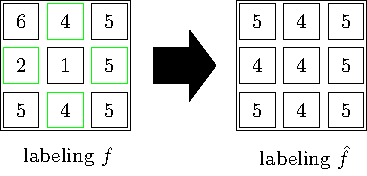
\includegraphics[width=.6\textwidth]{../figures/image_label/image_label.pdf}
        \caption{The left image with label $f$ is the input image. One algorithm could change the label of the image to the right image called $\hat f$. Green marked pixels are neighbours of the middle pixel.}
        \label{fig:img_label}
    \end{figure}
    Extending the previous notation we will use $\mathcal{P}_{\alpha, \beta}$ to express a set which only contains pixels which have the current label $\alpha$ or $\beta$.
    For example in \autoref{fig:img_label} $\mathcal{P}_{2,1}$ would be the set of the pixel in the middle and the left neighbour.\\
    In \autoref{fig:img_label} the green marked pixels are called neighbours of the pixel in the middle. If we write $\mathcal{N}$ then we mean the set of tuples of neighbours.
    So there would be four tuples where the middle pixel is in a tupel with the surrounding four. We add tuples for all neighbours in the whole image.
\section{Energy in images}
    Many computer vision problems can be formulated in a way that the energy in an image should be minimized. For example intensities of images are normally piecewise smooth but will chance their value
    rapidly at object boundaries. But intensity does also change if there is some noise at single pixels. To make a compromise of matching the original image but also achieving many areas of smooth 
    labels we can formulate the energy of an image:
    \begin{equation}
        E(f) = E_\text{smooth}(f) + E_\text{data}(f)
        \label{eq:ene}
    \end{equation}
    Here $f$ is the above mentioned labeling of all pixels in the image.
    $E_\text{data}$ is the part which cares about fitting the original image, $E_\text{smooth}$ considers the smooth parts.
   
    \subsection{Energy of data}
        Normally the data term is:
        \begin{equation}
            E_\text{data}(f) = \sum_{p \in \mathcal{P}} D_p(f_p)
        \end{equation}
        For $D_p$ often the quadratic norm is chosen, in image restoration it could be \\$(f_p -i_p)^2$ where $i_p$ is the original intensity of the pixel. However in my experiments a later presented energy function worked better.

    \subsection{Smoothness energy}
        The smoothness term can be defined in many possible ways. In most cases this frame is useful:
        \begin{equation}
            E_\text{smooth} = \sum_{ (p,q) \in \mathcal{N}} V_{p,q}(f_p, f_q)
        \end{equation}
        This term sums a potential function over all neighbours. 
        One could simply use $V_{p,q}(f_p, f_q) = K\cdot|f_p-f_q|$ but also $V_{p,q}(f_p,f_q) = \min(K, \lVert f_p-f_q \rVert)$ (with arbitrary constant $K$) and many others are possible. 
        % Depending on the energy function in practice you either choose the $\alpha$-$\beta$-swap oder $\alpha$-expansion algorithms.
        
\section{Label changing algorithms}
    In the following part we want to present you one of the main two algorithms for minimizing the energy in an image given in the paper \cite{paper}. 
    \subsection{$\alpha$-$\beta$-swap}
    The pure algorithm for optimizing a imagen via \abswap is given in \ref{alg:abswap}.
        \begin{algorithm}[h]
            \begin{algorithmic}[1]
                \Procedure{SwapMove}{$f$}
                \State $f \gets \textit{arbitrary labeling}$
                \State $s \gets 0$
                \For{ s = 1}
                    \State $s \gets 0$
                    \For{all $\{\alpha, \beta\}\subset \mathcal{L} $}
                        \State $\hat f \gets \arg\min E(f')$ within one \abswap
                        \If { $\hat E(\hat f)<E(f)$}
                            \State $f \gets \hat f$
                            \State $s \gets 1$
                        \EndIf
                    \EndFor
                \EndFor
                \State \Return{$f$}
                \EndProcedure
            \end{algorithmic}
            \caption{\abswap algorithm}
            \label{alg:abswap}
        \end{algorithm}
    The runtime is obviously in $\mathcal{O}(|\mathcal{L}|^2)$ and furthermore it can be proven that the algorithm converges after $\mathcal{O}(|\mathcal{P}|)$ cycles \cite{vekslerefficient}. One cycle is defined as line 6 to 10 in algorithm \ref{alg:abswap}.
    \noindent
    In line 6 we use the the \abswap to find the optimum. In the \abswap you only work with pixels in $\mathcal{P}_{\alpha,\beta}$. Changing only these pixels you want to find a new labeling
    which either asigns $\alpha$ or $\beta$ to the pixels. \autoref{fig:abswapchange} shows that if $\alpha=\text{red}$ and $\beta=\text{blue}$ only pixels of these two labels are touched. All pixels with other labels aren't changed
    in that cycle but will be changed in the next cycles if $\alpha$ and $\beta$ change. 
    \autoref{sec:imgtograph} will show which pixel receives which label.
    Which pixels receive which colours will be part of the \autoref{sec:imgtograph}.
    How to find the energy minimum via \abswap is explained in the following two sections.
    \begin{figure}[H]
        \centering
        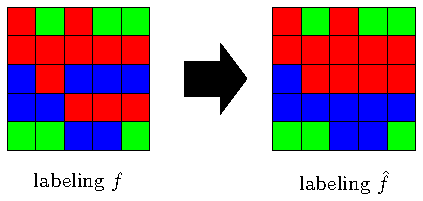
\includegraphics[width=.6\textwidth]{../figures/swap_change/swap_change.pdf}
        \caption{\abswap changes only red and blue pixels}
        \label{fig:abswapchange}
    \end{figure}

    
   \subsection{\aexp}
        For the \aexp a similar algorithm can be constructed. Due to page restrictions, this part is left out and can be found in \cite{paper}.
%        Algorithm \ref{alg:abexp} is similar to the previous one but we loop only over pixels since the \aexp move works different. This algorithms scales with $\mathcal{O}(|\mathcal{P}|)$. However we will see that line 7 will be more expensive.
%        \begin{algorithm}
%            \begin{algorithmic}[1]
%                \Procedure{ExpansionMove}{$f$}
%                \State $f \gets \textit{arbitrary labeling}$
%                \State $s \gets 1$
%                \For{ s = 1}
%                    \State $s \gets 0$
%                    \For{all $\alpha\in \mathcal{L} $}
%                        \State $\hat f \gets \arg\min E(f')$ within one \aexp
%                        \If { $\hat E(\hat f)<E(f)$}
%                            \State $f \gets \hat f$
%                            \State $s \gets 1$
%                        \EndIf
%                    \EndFor
%                \EndFor
%                \State \Return{$f$}
%                \EndProcedure
%            \end{algorithmic}
%            \caption{\aexp algorithm}
%            \label{alg:abexp}
%        \end{algorithm}\\
%    The \aexp is visually explained in \autoref{fig:aexpchange}. Instead of swapping pixel labels you extend the area of red pixels to other pixels. It is not allowed to change a red pixel to another color.
%    This would only possible if alpha is another label in the next cycle.
%    \begin{figure}[h]
%        \centering
%        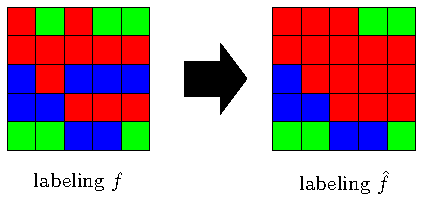
\includegraphics[width=.6\textwidth]{../figures/expansion_change/expansion_change.pdf}
%        \caption{\aexp only extend area of red pixels}
%        \label{fig:aexpchange}
%    \end{figure}




\section{From image to graph}
    \label{sec:imgtograph}
    Now we want to concentrate us now on the \abswap but for the \aexp the procedure is similar.
    \subsection{$\alpha$-$\beta$-swap}
        In \autoref{fig:graph} the constructed graph for a 1D-image is shown. In the first steps you add all pixels which have label $\alpha$ or $\beta$ as nodes to the graph. For the labels itself 
        you introduce two terminal nodes. Nodes which are neighbours in the original image are connected by an n-link. All nodes have an edge to the terminal nodes, called t-links. Note that there is no n-link w and y because they
        aren't neighbours, pixel x is between. But x hasn't label $\alpha$ or $\beta$ so it does not appear in the graph.

        \begin{figure}[h]
            \begin{subfigure}[t]{0.5\textwidth}
                \centering
                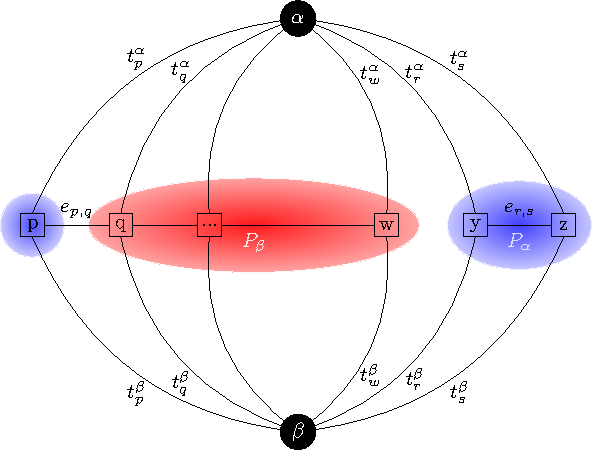
\includegraphics[width=1\textwidth]{../figures/pixel/pixel_skizze.pdf}
                \caption{Constructed graph of an 1D-image}
                \label{fig:graph}
            \end{subfigure}
            \begin{subfigure}[t]{0.5\textwidth}
                \centering
                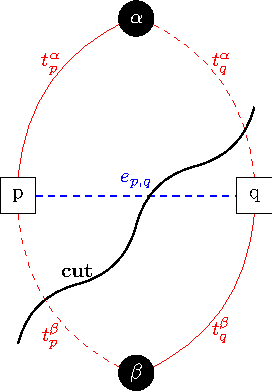
\includegraphics[width=.6\textwidth]{../figures/graph_cut/graph_1.pdf}
                \caption{Possible graph cut}
                \label{fig:cut}
            \end{subfigure}
            \caption{Graph and graph cut}
        \end{figure}
        \noindent 
        To include the information about the energy we add some edge weights which are given in \autoref{tab:weights}. 
        They are chosen like that to transform the energy minimizing problem into a graph-cut.
        \begin{table}[h]
            \centering
            \begin{tabular}{l l l}
                \textbf{edge}       & \textbf{weight}       & \textbf{for}\\[0.2cm]
                \hline \\[0.2cm]
                $t_p^\alpha$ \phantom{basdsadalub}        & $D_p(\alpha) + \sum\limits_{\small \substack{q \in \mathcal{N}_p \\q \notin \mathcal{P}_{\alpha,\beta}}} V_{p,q}(\alpha,f_q)$ \phantom{blubdasdsad} & $p \in \mathcal{P}_{\alpha,\beta}$ \\[0.9cm]
                $t_p^\beta$ \phantom{blub}        & $D_p(\beta) + \sum\limits_{\small \substack{q \in \mathcal{N}_p \\q \notin \mathcal{P}_{\alpha,\beta}}} V_{p,q}(\beta,f_q)$  & $p \in \mathcal{P}_{\alpha,\beta}$ \\[0.9cm]
                $e_{p,q}$    & $V_{p,q}(\alpha,\beta)$     & $\{p,q\} \in \mathcal{N} \wedge p,q \in \mathcal{P}_{\alpha,\beta}$
                \\[0.5cm] \hline
            \end{tabular}
            \caption{Edge weights for \abswap}
            \label{tab:weights}
        \end{table}
        
    % \subsection{$\alpha$-expansion}

\section{Minimum graph cut}
    In the previous section we saw how the graph was constructed. Now we want to show how we can find the minimum energy with graph cuts.
    
    \subsection{Procedure with graph cut}
        A cut \footnote{sometimes called s-t-cut or sink-flow-cut} on our graph means that there is no way from node $\alpha$ to node $\beta$. Minimum cut means that the sum of all cut edges weights must be minimal.
        One example of a cut is given in \autoref{fig:cut}. Depending on which of the t-links are cut, new labels for the pixels are assigned. In this example, p would have assigned the label $\beta$ and q $\alpha$. 
        In general, if the t-link from pixel p to $\alpha$ is cut then the new assigned label is $\alpha$. If the t-link to $\beta$ is cut then, label $\beta$ would be assigned.
    \subsection{Connection between energy and graph}
        In a mathematical formulation the cost of a cut can be expressed with
        \begin{equation}
           |\mathcal{C}| = \underbrace{\rule[-7.75mm]{0mm}{0mm} \sum_{p \in \mathcal{P}_{\alpha,\beta}} \left| \mathcal{C} \cap \{t_p^\alpha,t_p^\beta \} \right|}_{\text{cost of t-edges}}+ \underbrace{\sum\limits_{\small \substack{ \{p,q\} \in \mathcal{N}\\ \{p,q \} \subset \mathcal{P}_{\alpha,\beta}}} |\mathcal{C} \cap e_{p,q}|}_{\text{cost of n-links}}
        \end{equation}
        where $\mathcal{C}$ is the set of cut edges. This sum can be rewritten to 
        \begin{equation}
            |\mathcal{C}| = E(f^\mathcal{C}) - K.
        \end{equation}
        $K$ is a constant which is independent of the cut and $E(f^\mathcal{C})$ is the energy of the labling after the cut. One does see if we minimize the left term via the graph cut we find a minimum of the energy in the constructed graph. Note that this is not strictly a global minimum of the image and its labeling itself. However, it can be shown that it is within a known range of the optimum \cite{vekslerefficient}.


    \subsection{Finding a minimum cut}
        Quite a few algorithms exist in literature for the minimum graph cuts.
        One famous theorem is the \textit{Max-flow min-cut} which states that the maximum flow through a network is equivalent to 
        the cost of a minimum cut. Out of that the \textit{push-relabel} or \textit{Ford-Fulkerson} based algorithms were derived. 

\section{Implementation}
        For our graph structure Kolmogorov and Boykov showed that their algorithm works
        in practice faster than other known. The algorihtm and benchmarks can be found in \cite{expcomp} and \cite{thesis}. Kolmogorov himself also provides an fast \texttt{C++} implementation called \texttt{Maxflow}\footnote{\url{http://pub.ist.ac.at/~vnk/software.html}} \cite{kolmin}.
        I did also a small implementation \footnote{\url{https://github.com/roflmaostc/Fast-Approximate-Energy-Minimization-via-Graph-Cuts}} which uses \texttt{PyMaxflow}\footnote{\url{http://pmneila.github.io/PyMaxflow/}} for the graph cuts.
        The objective of our code was not speed and memory efficiency. It's only purpose was to test different energy functions on images to see the change in the results.


\section{Experiments}
    In our experiments we found out that using  $\hat D_p(f_p) = \sqrt{|f_p^2 - i_p^2|}$ and  $\hat V(f_p, f_q) = |f_p-f_q|$ delivered the best results.
    Choosing $\hat D_p$ can be motivated by the fact that the previous shown expressions for $D_p$ and $V(f_p,f_q)$ have a mismatch in scaling behaviour. The first scales quadratic the other linear.
    To eliminate this we choose $\hat D_p$ which scales linearly but also has a \textit{quadratic component}.
   
    \subsection{Example images}
    \autoref{fig:leopard} shows to the right the output image (produced with our \abswap implementation) using the classical euclidean energy function and the absolut different potential. The middle image
    is the output using our energy function. One can easily notice that the right image is very smooth and many parts of the originally structured skin is lost.
    \begin{figure}[H]
        \captionsetup[subfigure]{justification=centering}
        \begin{subfigure}{0.3\textwidth}
            \centering
            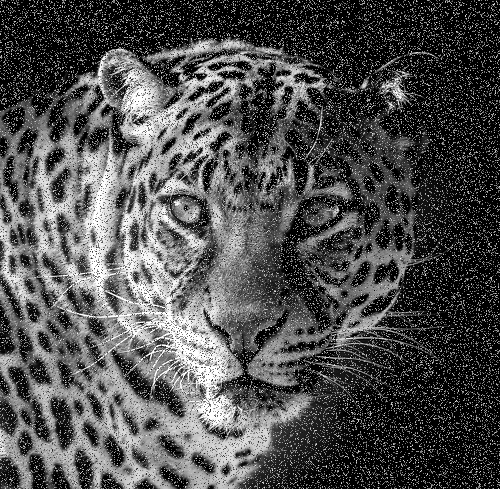
\includegraphics[width=.9 \textwidth]{../testimages/leopard/leopard_500_20percent.png}
            \caption{20\% noise \rule[-9.3mm]{0mm}{0mm}}
        \end{subfigure}
        \begin{subfigure}{0.3\textwidth}
            \centering
            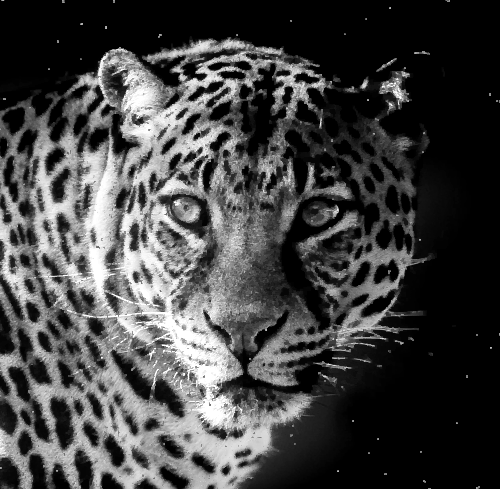
\includegraphics[width=.9\textwidth]{../testimages/leopard/500_20percent/denoised_leopard_500_20percent_10_cycle.png}
            \caption{10 cycles; $\hat D_p$; $\hat V$ \rule[-8.8mm]{0mm}{0mm}}
        \end{subfigure}
        \begin{subfigure}{0.3\textwidth}
            \centering
            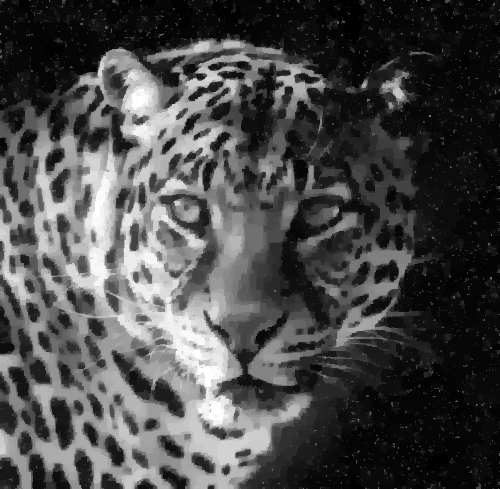
\includegraphics[width=.9\textwidth]{../testimages/leopard/v80_500_20/v80_bad_denoised_leopard_500_20percent_10_cycle.png}
            \caption{10 cycles; \\$D_p = (f_p-i_p)^2$; \\$V=80\cdot |f_p-f_q|$ }
        \end{subfigure}
        \caption{Comparison of different outputs of a noisy leopard}
        \label{fig:leopard}
    \end{figure}
    \noindent
    Using \autoref{eq:ene} it is also possible to print out the energy after every cycle. \autoref{plt:ene} shows that the biggest energy drop occurs always during the first cylce. Furthermore 
    the energy doesn't change much after the second and third cycle. This implies that in practice you shouldn't wait for convergence for a fast result but stop after a few cycles.
\begin{figure}[h]
        \begin{tikzpicture}
            \begin{axis}[
                width=12cm, height=7cm,
                xmin=-0.5, xmax=10.5, ymin=0, ymax=45000000,
                % y tick label style={/pgf/number format/fixed, /pgf/number format = \thinspace},
                scaled ticks=false,
                xtick = {0,1,2,3,4,5,6,7,8,9,10},
                y label style={at={(axis description cs:-0.05,.5)}},
                % ytick = {20000000,30000000,40000000},
                % ytick = {200000,400000, 600000, 800000},
                % yticklabels = {200000, 600000, 600000, 800000},
                xlabel = {Number of cycles}, ylabel = {Energy},
                minor y tick num = 4,
                legend entries = {House 20\% noise, Leopard 20\% noise, Lena 5\% noise}
            ]
            \addplot[color=blue, only marks, mark size = 1.5pt]
                table[x index = 0, y index = 1] {../testimages/houses/houses_500_20/houses_500_20percent_energie};

            \addplot[color=red, only marks, mark size = 1.5pt]
                table[x index = 0, y index = 1] {../testimages/leopard/500_20percent/leopard_500_20percent_energie};

            % \addplot[color=red, only marks, mark size = 1.5pt, mark=square]
            %     table[x index = 0, y index = 1] {../testimages/leopard/500_5percent/leopard_500_5percent_energie};
            
            \addplot[color=green, only marks, mark size = 1.5pt]
                table[x index = 0, y index = 1] {../testimages/Lena/500_5percent/Lenna_500_5percent_energy};
            
            %leopard 500
            \addplot[color=blue!100!black, domain=-1:12, line width=0.6pt] {4891040.0};

            %house
            \addplot[color=red!100!black, domain=-1:12, line width=0.6pt] {12374628.0};

            %lena 5percent
            \addplot[color=green, domain=-1:12, line width=0.6pt] {5445050.0};
            
            % \addplot[color=blue!60!black, domain=-1:10, line width=1pt] {12374628.0};

            % \addplot[color=blue, only marks, mark size = 1.5pt]
            %     table[x index = 0, y index = 1] {../testimages/Lena/500_10percent/Lenna_500_10percent_energy};
            % \addplot[color=red, only marks, mark size = 1pt]
            %     table[x index = 0, y index = 1] {../testimages/dog2/2_output.txt};
            % \draw[color=green!40!black] (axis cs:-1,3551258) -- node[below]{Unnoised image} (axis cs:9,3551258);
            % \addplot[color=red, only marks, mark size = 1.5pt]
            %     table[x index = 0, y index = 1] {../testimages/leopard/250_10percent/250_10percent};
            % \addplot[color=red!60!black, domain=-1:10, line width=1pt] {3551258};
            
            % \addplot[color=green, only marks, mark size = 1.5pt]
            %     table[x index = 0, y index = 1] {../testimages/Lena/200_5percent/200_5percent.txt};
            % \addplot[color=green!60!black, domain=-1:10, line width=1pt] {1499586};
            \end{axis}
        \end{tikzpicture}
        \caption{Energy over cycles obtained by our implementation. The horizontal lines are the energy of the original, clean image}
        \label{plt:ene}
    \end{figure}


 
     \begin{figure}[H]
        \captionsetup[subfigure]{justification=centering}
        \begin{subfigure}{0.3\textwidth}
            \centering
            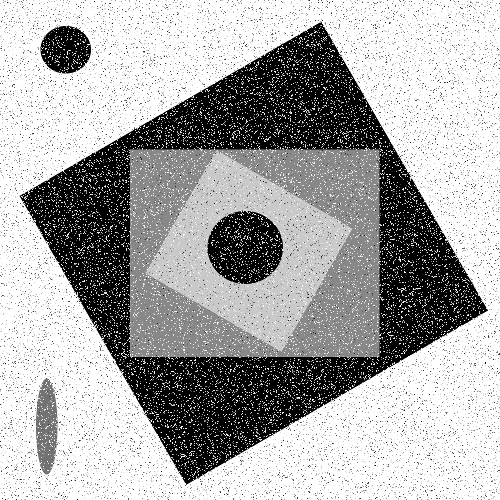
\includegraphics[width=.9 \textwidth]{../testimages/shapes/shapes_500_15percent.png}
            \caption{15\% noise \rule[-9.3mm]{0mm}{0mm}}
        \end{subfigure}
        \begin{subfigure}{0.3\textwidth}
            \centering
            
\includegraphics[width=.9\textwidth]{../testimages/shapes/shapes_500_15percent/denoised_shapes_500_15percent_10_cycle.png}
            \caption{10 cycles; $\hat D_p$; $\hat V$ \rule[-8.8mm]{0mm}{0mm}}
        \end{subfigure}
        \begin{subfigure}{0.3\textwidth}
            \centering
            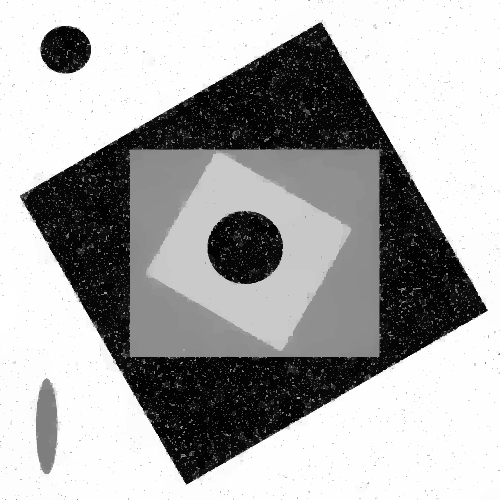
\includegraphics[width=.9\textwidth]{../testimages/shapes/shapes_500_15_min_500_euclidean/min_500_euclidean_bad_denoised_shapes_500_15percent_10_cycle.png}
            \caption{10 cycles; \\$D_p = (f_p-i_p)^)$; \\$V=\max \left(500,(f_p-f_q)^2\right)$ }
        \end{subfigure}
        \caption{Comparison of different outputs}
        \label{fig:leopard}
    \end{figure}

   
\section{Conclusion}
    Graph-cuts are still state of the art in computer vision because they can minimize the energy in the whole image and not only piecewise.
    However today the \aexp algorithm is used more because in total you have far less graph cuts to find. 
    Doing the \abswap for grayscale images you've already got $\approx 30000$ iterations due to the swap of all different pairs of labels. Furthermore, in each swap
    the graphs are constructed and a minimum cut has to be found. The \aexp has bigger graphs but only a few hundred which is much less.
    Excluding deep learning graph cuts in computer vision are still a very interesting topic for doing task like segmentation.

%------------------------- REFERENCES -------------------------%
\printbibliography
\end{document}
